\section{Coding Ladder Lotteries}
In the paper Coding Ladder Lotteries, written by Aiuchi, Yamanaka, Hirayama and Nishitani, the authors provide three methods to encode ladder lotteries as 
binary strings~\cite{A5}. Coding discrete objects as binary strings is an appealing theme because 
it allows for compact representation of them for a computer~\cite{A5}.
\subsection{Route Based Encoding}
The first method is termed \emph{route based encoding method} in 
which each route of an element in the permutation has a binary encoding. Let $l$
be a ladder lottery for some arbitrary permutation $\pi$ of order $n$. The route 
of element $p_{i}$ is encoded by keeping in mind $p_{i}$ crosses bars in its route 
going left zero or more times and crosses bars in its route going right zero or 
more times~\cite{A5}. The maximum number of bars $p_{i}$ can have is $n-1$, therefore the 
upper bound for the number of left/right crossings for $p_{i}$ is $n-1$~\cite{A5}. 
Let a left crossing be denoted with a $'0'$ and let a right crossing be denoted 
with a $'1'$. Let $C(p_{i})$ be the route encoding for the $i^{th}$ element 
in $\pi$. To construct $C(p_{i})$,  append $0$ and $1$ to each other representing 
the left and right crossings of $p_{i}$ from the top left 
to bottom right of the ladder~\cite{A5}. If the number of crossings for $p_{i}$ 
is less than $n-1$, append $0s$ to the encoding of the route of $p_{i}$ until
the encoding is of length $n-1$~\cite{A5}. Let $RC(l)$ be the route encoding for 
some arbitrary ladder in $OptL\{\pi\}$. $RC(l)$ is $C(p_{1}), C(p_{2}), \dots C(p_{n})$.
For an example of the route encoding for the root ladder of $(3,2,5,4,1)$ refer to 
Figure~\ref{fig:route-encoding}. In~\ref{fig:route-encoding} you will see that $C(p_{1})$ is 11\underline{00}. Underlined 
$0s$ are the $0s$ added to ensure the length of $C(p_{1})$ is $n-1$.
Since the length of $C(\pi)$ is $n-1$ and the number of elements in $\pi$ is $n$
then the length of $RC(l)=n(n-1)$. Hence the number of bits needed for $RC(l)$ 
belongs to $\mathcal{O}(n^{2})$.\par 
\begin{figure}[!htp]
    \begin{center}
        \begin{tikzpicture}
    
            %%draw the lines
            \draw(0, 0) to (0, 4);
                \node at(0, 4.3){3};
                \node at(0, -0.3){1};
            \draw(2, 0) to (2, 4);
                \node at (2, 4.3){2};
                \node at(2, -0.3){2};
            \draw(4, 0) to (4, 4);
                \node at (4, 4.3){5};
                \node at (4, -0.3){3};
            \draw(6, 0) to (6, 4);
                \node at (6, 4.3){4};
                \node at (6, -0.3){4};
            \draw(8, 0) to (8, 4);
                \node at (8, 4.3){1};
                \node at (8, -0.3){5};
    
            %%Draw the bars
            \draw(0, 2) to (2, 2);
            \draw(2, 1.5) to (4,1.5);
            \draw(0, 1) to (2, 1);

            \draw(4, 3) to (6, 3);
            \draw(6, 2.5) to (8, 2.5);
            \draw(4, 2) to (6, 2);
        \end{tikzpicture}
    \end{center}
   
 \caption{The route encoding for the following ladder lottery is \newline 11\underline{00}01\underline{00}11\underline{00}01\underline{00}0000}
 \label{fig:route-encoding}

\end{figure}

\subsection{Line Based Encoding}
The second method is termed \emph{line based encoding} which focuses 
on encoding the lines of the ladder lottery. Each line is represented 
as a sequence of endpoints of bars. Let $l$ be an optimal ladder lottery 
with $n$ lines and $b$ bars, then for some arbitrary line, $i$, there 
are zero or more right/left endpoints of bars that 
come into contact with $i$~\cite{A5}. Let $LC(i)$ denote the line based encoding for line $i$.
Let $1$ denote a left end point that 
comes into contact with line $i$ and let $0$ denote a right 
end point that comes into contact with line $i$. Finally, append a $0$
to line $i$ to denote the end of the line. Then line $i$ can be 
encoded, from top to bottom, as a sequence of $1s$ and $0s$ that 
terminates in a $0$.  Given the ladder in Figure~\ref{fig:line-encoding}, 
$LC(3)$ is $001\underline{0}$. The \underline{0} denotes 
the end of the line. Let $LC(l)$ be the line encoding for 
some arbitrary ladder, then $LC(l)=LC(1), LC(2), \dots LC(n)$.
Let $l(4,2,3,1)$ refer to the ladder in Figure~\ref{fig:line-encoding}, then 
$LC(l(4,2,3,1))=11\underline{0}010\underline{0}110\underline{0}010\underline{0}0\underline{0}$.
\begin{figure}[h]
    \begin{center}
        \begin{tikzpicture}
            \draw(0, 0) to (0, 4);
            \node at (0, 4.3){4};
            \node at (0, -0.3){1};
        \draw(2, 0) to (2, 4);
            \node at (2, 4.3){2};
            \node at (2, -0.3){2};
        \draw(4, 0) to (4, 4);
            \node at (4, 4.3){3};
            \node at (4, -0.3){3};
        \draw(6, 0) to (6, 4);
            \node at (6, 4.3){1};
            \node at (6, -0.3){4};

        %%bars 
        \draw(0, 3) to (0.7, 3);
            \node at (0.35, 3.3){1};
        \draw (1.3, 3) to (2, 3);
            \node at (1.65, 3.3){0};

        \draw(2, 2.5) to (2.7, 2.5);
            \node at (2.35, 2.8){1};
        \draw(3.3, 2.5) to (4, 2.5);
            \node at (3.65, 2.8){0};

        \draw(4, 2) to (4.7, 2);
            \node at (4.35, 2.3){1};
        \draw(5.3, 2) to (6, 2);
            \node at (5.65, 2.3){0};

      

        \draw(2, 1) to (2.7, 1);
            \node at (2.35, 1.3){1};
        \draw(3.3, 1) to (4, 1);
            \node at (3.65, 1.3){0};

        \draw(0, 0.5) to (0.7, 0.5);
            \node at (0.35, 0.8){1};
        \draw(1.3, 0.5) to (2, 0.5);
            \node at (1.65, 0.8){0};

        \end{tikzpicture}
      

    \end{center}
    \caption{$LC(l(4,2,3,1))=11\underline{0}0110\underline{0}010\underline{0}0$}
    \label{fig:line-encoding}
\end{figure}
 
In order to reconstruct $l$ from its $LC(l)$, or in other words decode
$LC(l)$ it is important to recognize that the first line only has left endpoints attached to it
\cite{A5}. Since left end points are encoded as a $1$ then it is guaranteed that the first $0$ 
represents the end of line $1$. Secondly, the last/$nth$ line 
has only right end points attached to it.  Therefore $LC(i=n)$ will only have $0s$. Therefore, $LC(i=n)$
does not require a terminating $0$. Thirdly, for any 
line $i+1$, if line $i+1$ has a $0$ then there must be a corresponding $1$
in line $i$. That is to say, if the right end point of a bar is on line 
$i+1$ then that same bar must have a left endpoint on line $i$. To decode 
$LC(l)$ start by decoding line $1$. The line will contain $0$ or more 
left end points. To decode $LC(i+1)$ where $i+1>1$, go to 
$LC(i)$ and match each $1$ in $LC(i)$ with a $0$ in $LC(i+1)$. 
Let $k=$ the number of $1s$ in $LC(i)$. Let $j=$ the number 
of $0s$ in $LC(i+1)$ then $k=j-1$; due to the last $0$ in $LC(i+1)$ denoting 
the end of line $i+1$.  Intuitively, this means match every left end point 
of a bar in line $i$ with a right end point in line $i+1$. The last $0$
represents the end of line $i+1$. For an example of a full decoding of $LC(l(4,2,3,1))$
please refer to Figure~\ref{fig:line-encoding}.\par 

Since each bar is encoded as two bits, and there are $n-1$ bits as terminating bits; 
one for each line in $l$, then the number of bits required is $n + 2b -1$, where $n$
is the number of lines and $B$ is the number of bars~\cite{A5}. Encoding and decoding can be 
done in $\mathcal{O}(n+b)$ time~\cite{A5}. Clearly the line-based encoding 
trumps the route-based encoding in both time and space complexity.

\subsection{Improved Line-Based Encoding}
Although the line-based encoding is better than the route based 
encoding, it can still be further optimized. The authors provide 
three improvements to the line-based encoding. These three improvements
can be combined to really help improve the line based encoding's 
space efficiency~\cite{A5}. 
\subsubsection{Improvement 1}
Since the $nth$ line has only right endpoints attached to it, 
then it actually does not need to be encoded. Right endpoints 
are denoted as $0$ and left endpoints are encoded as $1$, therefore the number of right endpoints 
for line $n$ is equal to the number of $1s$ in $LC(i=n-1)$.
Thus, there is no need for $LC(i=n)$~\cite{A5}. The encoding with improvement 
one for the ladder in Figure~\ref{fig:line-encoding} is $11\underline{0}0110\underline{0}010$.
\subsubsection{Improvement 2}
Improvement two is based off of the fact that for any two bars,
$x,y$, let $l_{x}$ denote the left endpoint of bar $x$, let 
$l_{y}$ denote the left endpoint of bar $y$, let $r_{x}$ denote 
the right end point of bar $x$ and let $r_{y}$ denote the right 
end point of bar $y$. Let line $i$ be the line of $l_{x}$ and $l_{y}$
and let line $i+1$ be the line of $r_{x}$ and $r_{y}$.
\begin{lemma}
There are three possible cases for the placement of $x$ and $y$ in some arbitrary ladder from $OptL\{\pi\}$. 
The first case is that there 
is at least one other bar, $z$, with a right end point, $r_{z}$ between $l_{x}$
and $l_{y}$ on line $i$. The second case is that there is at least one other bar 
$z$, with a left end point, $l_{z}$, between $r_{x}$ and $r_{y}$ on line $i+1$. 
The third case is that there is at least one bar, $z$, with a right end point, 
$r_{z}$, between $l_{x}$ and $l_{y}$ on line $i$ and there is at least one other bar, 
$z\prime$ with a left end point, $l_{z\prime}$, between $r_{x}$ and $r_{y}$ on line $i+1$~\cite{A5}. 
For an example of all three cases refer to Figure~\ref{fig:three-cases}\par
\end{lemma}
%%figure demonstrating the three cases for bar positions
\begin{figure}[h]
       
            %%first case
            \begin{minipage}{.3\textwidth}
                \begin{tikzpicture}
                    \draw(0, 0) to (0, 4);
                        \node at (2, 4.3){\small{$i+1$}};
                    \draw(1, 0) to (1, 4);
                        \node at (1, 4.3){\small{$i$}};
                    \draw(2, 0) to (2, 4);
                        \node at (0, 4.3){\small{$i-1$}};
                    \draw(0, 2) to (1, 2);
                        \node at (.5, 2.3){\small{$r_{z}$}};
                    \draw(1, 3) to (2, 3);
                        \node at (1.5, 3.3){\small{$l_{x}$}};
                    \draw(1, 1) to (2, 1);
                        \node at (1.5, 1.3){\small{$l_{y}$}};
                \end{tikzpicture}
            \end{minipage}
              \begin{minipage}{.3\textwidth}

                 \begin{tikzpicture}
                
                  \draw(0, 0) to (0, 4);
                     \node at (0, 4.3){\small{$i-1$}};
                  \draw(1, 0) to (1, 4);
                    \node at (1, 4.3){\small{$i$}};
                  \draw(2, 0) to (2, 4);
                     \node at (2, 4.3){\small{$i+1$}};
                   \draw(0, 3) to (1, 3);
                         \node at (.5, 3.3){\small{$r_{x}$}};
                    \draw(1, 2) to (2, 2);
                         \node at (1.5, 2.3){\small{$l_{z}$}};
                     \draw(0, 1) to (1, 1);
                         \node at (0.5, 1.3){\small{$r_{y}$}};
                
                   
                
                \end{tikzpicture}
             \end{minipage}
             \begin{minipage}{.3\textwidth}

                \begin{tikzpicture}
                
                 \draw(0, 0) to (0, 4);
                    \node at (1, 4.3){\small{$i$}};
                 \draw(1, 0) to (1, 4);
                    \node at (2, 4.3){\small{$i+1$}};
                 \draw(2, 0) to (2, 4);
                    \node at (0, 4.3){\small{$i-1$}};
                 \draw(3, 0) to (3, 4);
                    \node at (3, 4.3){\small{$i+2$}};
                    \draw(1, 3) to (2, 3);
                        \node at (1.3, 3.3){\small{$l_{x}$}};
                        \node at (1.7, 3.3){\small{$r_{x}$}};
                     \draw(0, 2) to (1, 2);
                        \node at (0.7, 2.3){\small{$r_{z}$}};
                    \draw(1, 1) to (2, 1);
                        \node at (1.3, 1.3){\small{$l_{y}$}};
                         \node at (1.7, 1.3){\small{$r_{y}$}};
                     \draw(2, 2) to (3, 2);
                        \node at (2.3, 2.3){\small{$l_{z\prime}$}};
                
                   
                
                \end{tikzpicture}
            \end{minipage}
        

    \caption{Three examples of the three cases for the placement 
    of bars $x$ and $y$ in a ladder lottery}
    \label{fig:three-cases}
\end{figure}

\begin{proof}
    Suppose that none of the above cases hold. Let $l$ be an 
    optimal ladder lottery with bars $x$ and 
    bar $y$. If none of the cases hold then $x$ and $y$ are directly above/below each other without 
    the endpoint of some third bar $z$ between $l_{x}$ and $l_{y}$ or between $r_{x}$ and $r_{y}$.
    Let $x$ be the bar for the inversion of two elements $p_{i}$ and $p_{j}$ in $\pi$. 
    As $p_{i}$ and $p_{j}$ travel through the ladder they will cross each other at bar $x$; 
    thus uninverting them. Since bar $y$ is directly below bar $x$, then $p_{i}$ and $p_{j}$ will cross 
    bar $y$ thus re-inverting them. Therefore, there will need to be a third 
    bar that uninverts $p_{i}$ and $p_{j}$ a second time. Since this third bar is 
    redundant, $l$ is non-optimal which is a contradiction. Let $x$ be a bar for two 
    elements in $\pi$, $p_{i}$ and $p_{j}$ such that $p_{i}$ and $p_{j}$ do not form an inversion. Then $x$ 
    will transpose $p_{i}$ and $p_{j}$ and $y$ will transpose them a second time. Thus making both $x$ and $y$ redundant
    bars which is also a contradiction. Therefore one of the above cases must hold.
\end{proof}



Knowing that one of the three above cases must hold is beneficial for improving the 
line-based encoding. If $l_{x}$ and $l_{y}$ on line $i$ have no $r_{z}$ between them, 
then there must be at least one $l_{z\prime}$ between $r_{x}$ and $r_{y}$ on line $i+1$.
Since a left endpoint is encoded as a $1$ and a right endpoint is encoded as a $0$, 
a $1$ can be omitted for the encoding of line $i+1$ if $l_{x}$ and $l_{y}$ have no $r_{z}$
between them on line $i$~\cite{A5}. That is to say, if there is not a $0$ between 
the two  $1s$ for $l_{x}$, $l_{y}$ in $LC_{i}$, it is implied that there is at least one $1$ between 
the two $0s$ for $r_{x}$, $r_{y}$ on $LC_{i+1}$. Hence, one of the $1s$ in $LC(i+1)$ can be omitted. 
The line encoding with improvement two for the ladder in Figure~\ref{fig:line-encoding} is $11\underline{0}010\underline{0}00\underline{0}0$.
\subsubsection{Improvement 3}
Improvement three is based off of saving some bits for right 
end points/$0s$ in $LC(i=n-1)$. Since line $n$ has no left end points,
then there must be some right endpoints between any two 
consecutive bars connecting lines $n-1$ and line $n$. If you 
refer to Figure~\ref{fig:improvement3}, then the only configuration for lines $n-2, n-1, n$
is the middle configuration~\cite{A5}. Knowing this, then 
given two bars, $x$ and $y$ with $l_{x}$/$l_{y}$ on line 
$n-1$ and $r_{x}$/$r_{y}$ on line $n$, there must be at least 
one bar, $z$, with its $r_{z}$ between $l_{x}$ and $l_{y}$
on line $n-1$. Thus, for every $1$ in $LC(i=n-1)$ except the 
last $1$ a $0$ must immediately proceed any $1$. 
Since this $0$ is implied, it can be removed from $LC(i=n-1)$~\cite{A5}. 
For an example of improvement three with its line encoding for $LC(i=n-1)$ please refer to Figure~\ref{fig:improvement3}.
\begin{figure}[h]
    \centering
    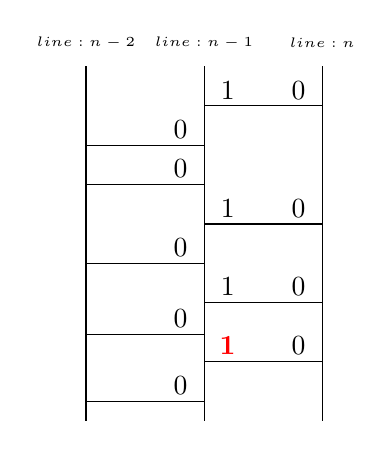
\begin{tikzpicture}
        \draw(0, -0.5) to (0, 4);
            \node at (0, 4.3){\tiny{$line:n-2$}};
            \draw(0, 3) to (1.5, 3);
                \node at (1.2, 3.2){$0$};
            \draw(0, 2.5) to (1.5, 2.5);
                \node at (1.2, 2.7){$0$};
            \draw(0, 1.5) to (1.5, 1.5);
                \node at (1.2, 1.7){$0$};
            \draw(0, 0.6) to (1.5, 0.6);
                 \node at (1.2, 0.8){$0$};
            \draw(0, -0.25) to (1.5, -0.25);
                \node at (1.2, -0.05){$0$};
        \draw(1.5, -0.5) to (1.5, 4);
            \node at (1.5, 4.3){\tiny{$line:n-1$}};
            \draw(1.5, 3.5) to (3, 3.5);
                \node at (1.8, 3.7){$1$};
                \node at (2.7, 3.7){$0$};
            \draw(1.5, 2) to (3, 2);
                \node at (1.8, 2.2){$1$};
                \node at (2.7, 2.2){$0$};
            \draw(1.5, 1) to (3, 1);
                \node at (1.8, 1.2){$1$};
                \node at (2.7, 1.2){$0$};
            \draw(1.5, 0.25) to (3, 0.25);
                \node at (1.8, 0.45){$\textcolor{red}{\textbf{1}}$};
                \node at (2.7, 0.45){$0$};

        \draw(3, -0.5) to (3, 4);
            \node at (3, 4.3){\tiny{$line:n$}};
    \end{tikzpicture}
    \caption{The line coding for $LC(i=n-1)$ with improvement three is $101110$\underline{$0$}. The red, bold $1$ represents 
    the last left end point in $LC(i=n-1)$, therefore the proceeding $0$ must be 
    included in $LC_{n-1}$. For every other $1$ in $LC(i=n-1)$, a $0$ is omitted following 
    said $1$.}
    \label{fig:improvement3}
\end{figure}
\subsubsection{Combining All Three}
The combination of all three improvements can be done independently.\newline 
Let $IC(l(4,2,3,1))$ be the \emph{improved line-based encoding} for $l(4,2,3,1)$ 
by applying improvements 1-3 to $LC(l(4,2,3,1))$. Recall that $LC(l)$ denotes the line-based encoding for some ladder $l$.
The $LC(l(4,2,3,1))$ for the ladder in Figure~\ref{fig:line-encoding} is $11\underline{0}10101\underline{0}0010101\underline{0}000$.
By applying improvement one, we get $11\underline{0}101011\underline{0}0010101\underline{0}$. 
Notice how the last three $0s$ from $LC(l(4,2,3,1))$ were removed because they represented $LC(i=n)$.
By applying improvement two to improvement one we get $11\underline{0}10011\underline{0}001001\underline{0}$.
Notice how the second, and eighth $1$ were removed because they are implied by 
the successive $0s$. By applying improvement three to the result of improvement 
two we get $11\underline{0}10011\underline{0}00101\underline{0}$. Notice how the last $0$ 
was removed from improvement two. This is because the $0$ is implied in $LC(i=n-1)$
due to the configuration between of bars connecting lines $n-1$ and line $n$. The $IC(l(4,2,3,1))$ for the ladder in Figure~\ref{Fig:allthree} 
is $IC(l(4,2,3,1))=11\underline{0}10011\underline{0}00101\underline{0}$.\pagebreak

\begin{figure}[!htp]
     \centering
    \begin{tikzpicture}
         \draw(0, 0) to (0, 4);
             \node at (0, 4.3){\tiny{$line:n-3$}};
             \draw(0, 3.5) to (1.5, 3.5);
             \draw(0, 2.5) to (1.5, 2.5);
         \draw(1.5, 0) to (1.5, 4);
             \node at (1.5, 4.3){\tiny{$line:n-2$}};
             \draw(1.5, 3) to (3, 3);
             \draw(1.5, 3.8) to (3, 3.8);
             \draw(1.5, 2) to (3, 2);
             \draw(1.5, 1) to (3, 1);
         \draw(3, 0) to (3, 4);
             \node at(3, 4.3){\tiny{$line:n-1$}};
             \draw(3, 2.5) to (4.5, 2.5);
             \draw(3, 1.5) to (4.5, 1.5);
             \draw(3, 0.5) to (4.5, 0.5);
         \draw(4.5, 0) to (4.5, 4);
             \node at(4.5, 4.3){\tiny{$line:n$}};
     \end{tikzpicture}
     \caption{A ladder used to illustrate all three improvements $IC(l)$. 
     \newline $IC(l)=11\underline{0}10011\underline{0}00101\underline{0}$}
     \label{Fig:allthree}
\end{figure}